\subsection{Gluing Column Extrusions together with Strip Connectors}
\label{sec:strip_connectors}

Now that all the column extrusions $\left\{ \mathcal C^{(i)} \right\}$ have the same evolution time,
we would like to glue them together into a continuous strip of paper.
In order to achieve this, we consider the time-axis boundaries of $\mathcal C^{(i)}$
(red line in Figure~\ref{fig:level_shift}~\ref{fig:up_down}).
\graphicspath{{./figures/}}
\begin{wrapfigure}{r}{0.35\textwidth}
    \def\svgwidth{0.35\textwidth}
    \input{./figures/boundaries.pdf_tex}%
    \caption{Boundaries of adjacent column extrusions with $D_j = 8\epsilon$}
    \label{fig:boundaries}
\end{wrapfigure}
\begin{itemize}
    \item During the horizontal evolution of any row $j$, both boundaries move along the positive $y$-axis with unit velocity
          (Figure~\ref{fig:level_shift0}~\ref{fig:level_shift3}~\ref{fig:level_shift4}~\ref{fig:up_down0}~\ref{fig:up_down4}~\ref{fig:up_down5}).
    \item During the vertical transition from row $j$ to $j+1$, both boundaries move back and forth along the $x$-axis with unit velocity.
          (Figure~\ref{fig:level_shift1}~\ref{fig:level_shift2}~\ref{fig:up_down1}~\ref{fig:up_down2}~\ref{fig:up_down3}).
          We can divide the vertial transition into $k = D_j/(2\epsilon)$ intervals of length $2\epsilon$.
          Each of these interval segments is either a up-shift, a down-shift, or a up-down gadget.
    \begin{itemize}
        \item In the first half of each interval ($\epsilon$ time), the left and right boundaries move towards each other;
              i.e. the left boundary moves along the positive $x$-axis, and the right boundary moves along the negative $x$-axis for a distance of $\epsilon$.
        \item In the second half of each interval, the left and right reverse directions, and return to their original positions.
        \item After $D_j$ time, the boundaries return to their original positions, and resume their movement in the positive $y$ direction.
    \end{itemize}
\end{itemize}

\graphicspath{{./figures/}}
\begin{figure}[htb]
    \def\svgwidth{1.1\textwidth}
    \input{./figures/connector_cross_section.pdf_tex}%
    \caption{
    Cross section evolution of column connector gadget.
    }
    \label{fig:connector_cross_section}
\end{figure}

\begin{figure}[!htb]
\graphicspath{{figures/column_connector}}
    \centering
    \subfloat[Initial height.]{
        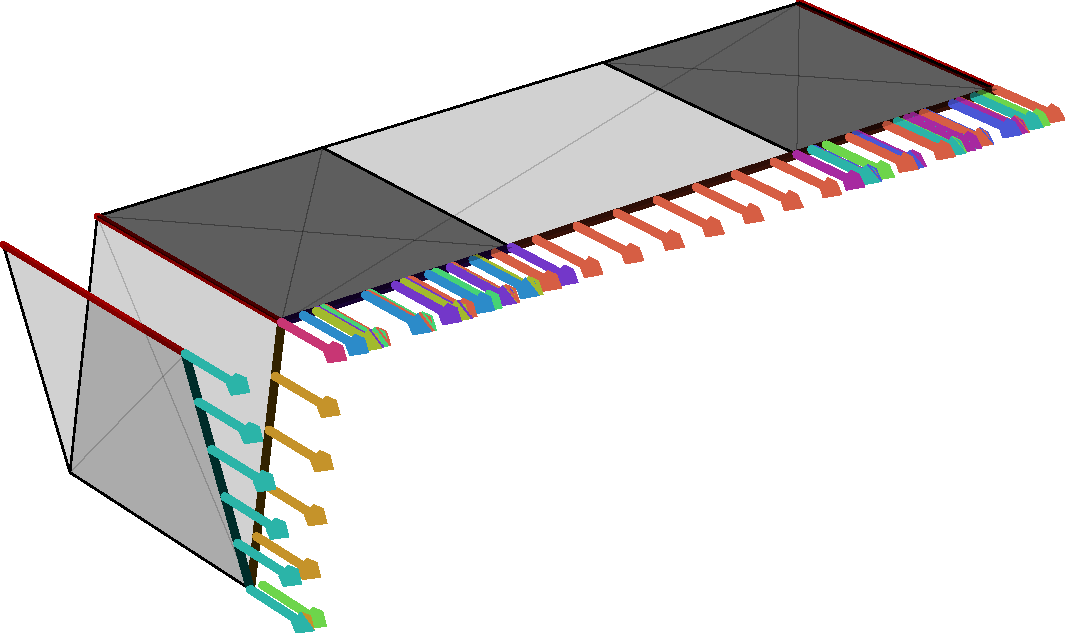
\includegraphics[width=0.23\textwidth]{figures/column_connector/column0.pdf}
    }%
    \subfloat[Connector moves outwards.]{
        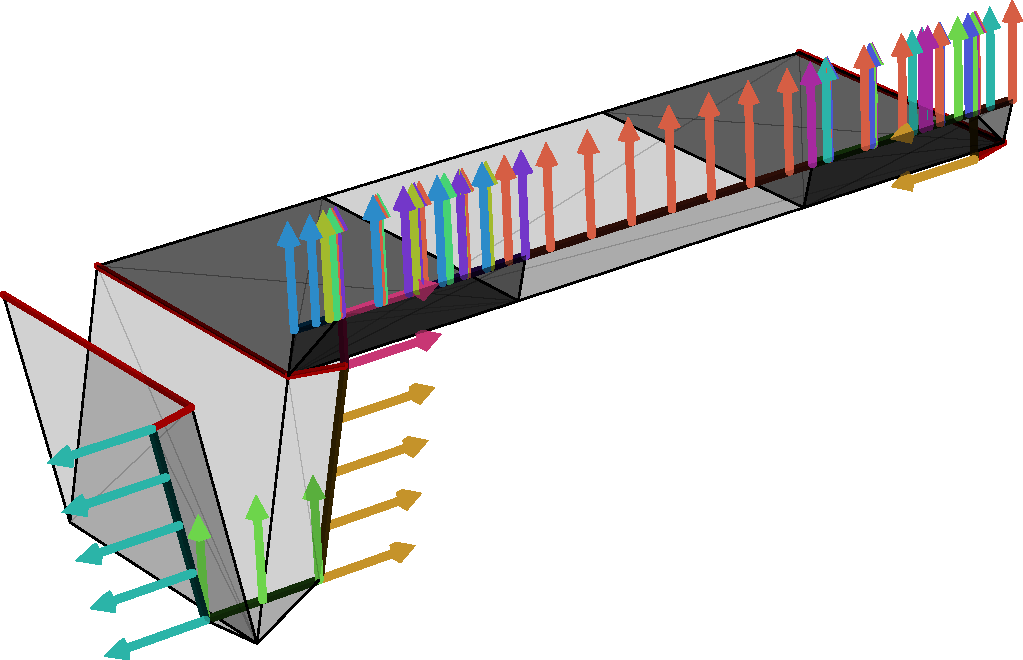
\includegraphics[width=0.21\textwidth]{figures/column_connector/column1.pdf}
    %}
    %\subfloat[]{
        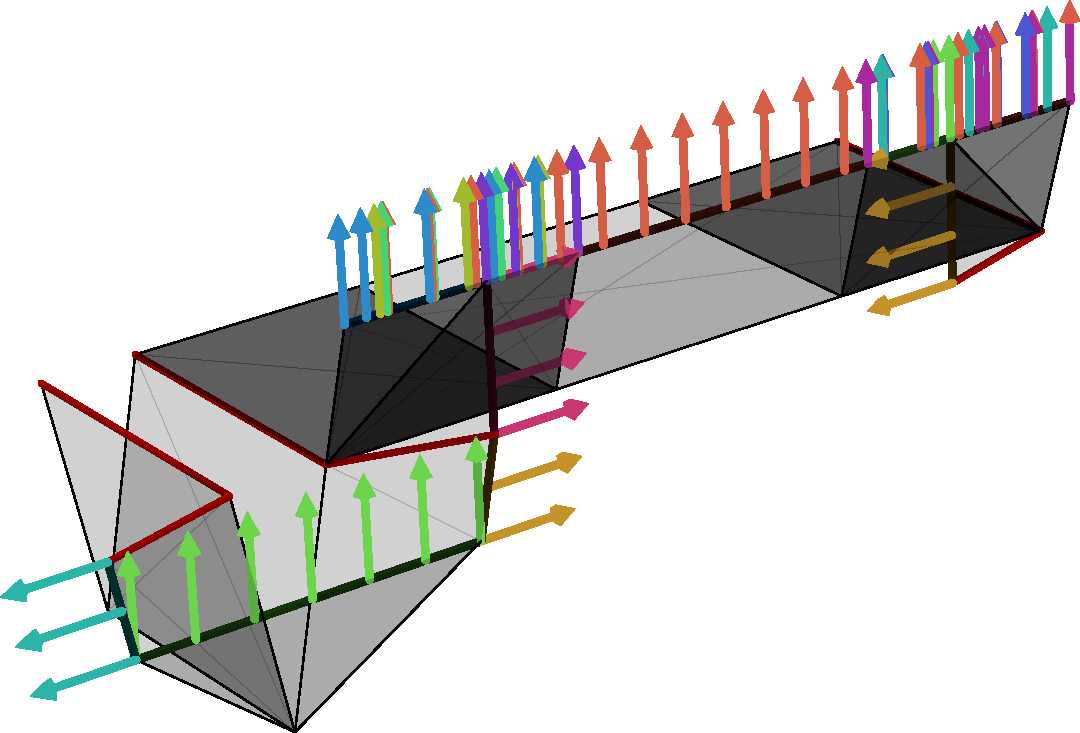
\includegraphics[width=0.21\textwidth]{figures/column_connector/column2.pdf}
    }%
    \subfloat[Connector at maximum width.]{
        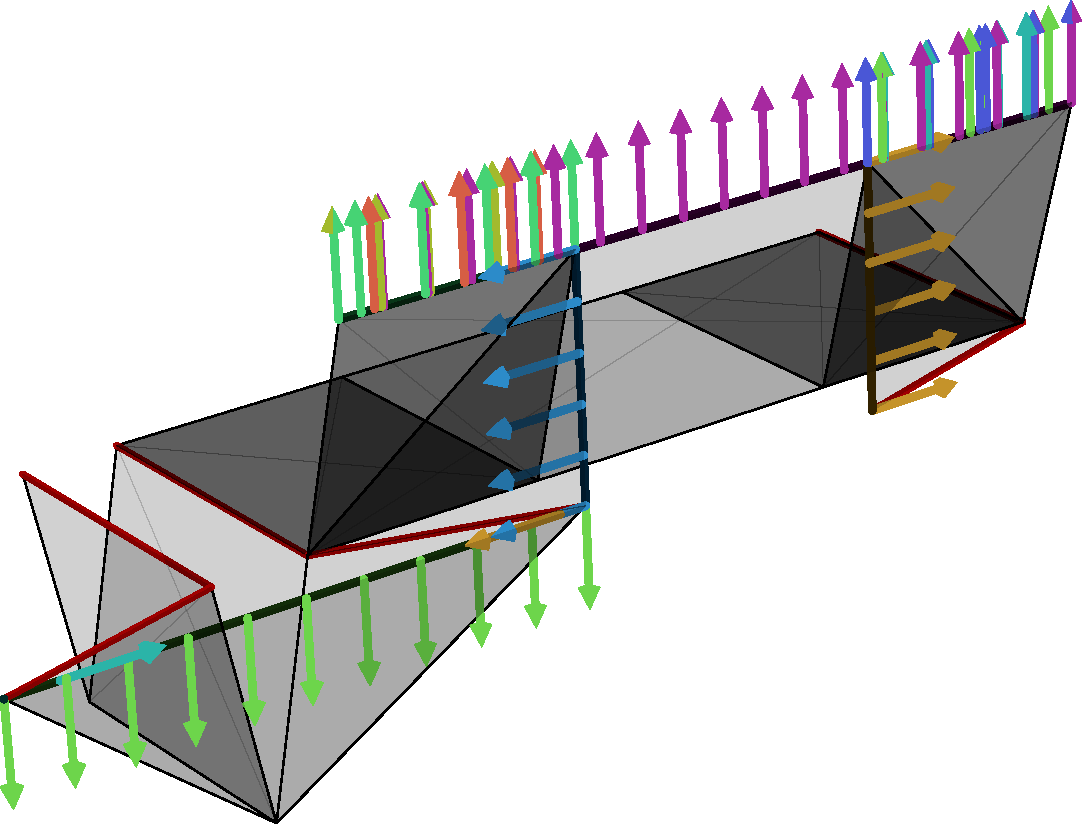
\includegraphics[width=0.24\textwidth]{figures/column_connector/column3.pdf}
    }%

    \subfloat[Connector moves inwards.]{
        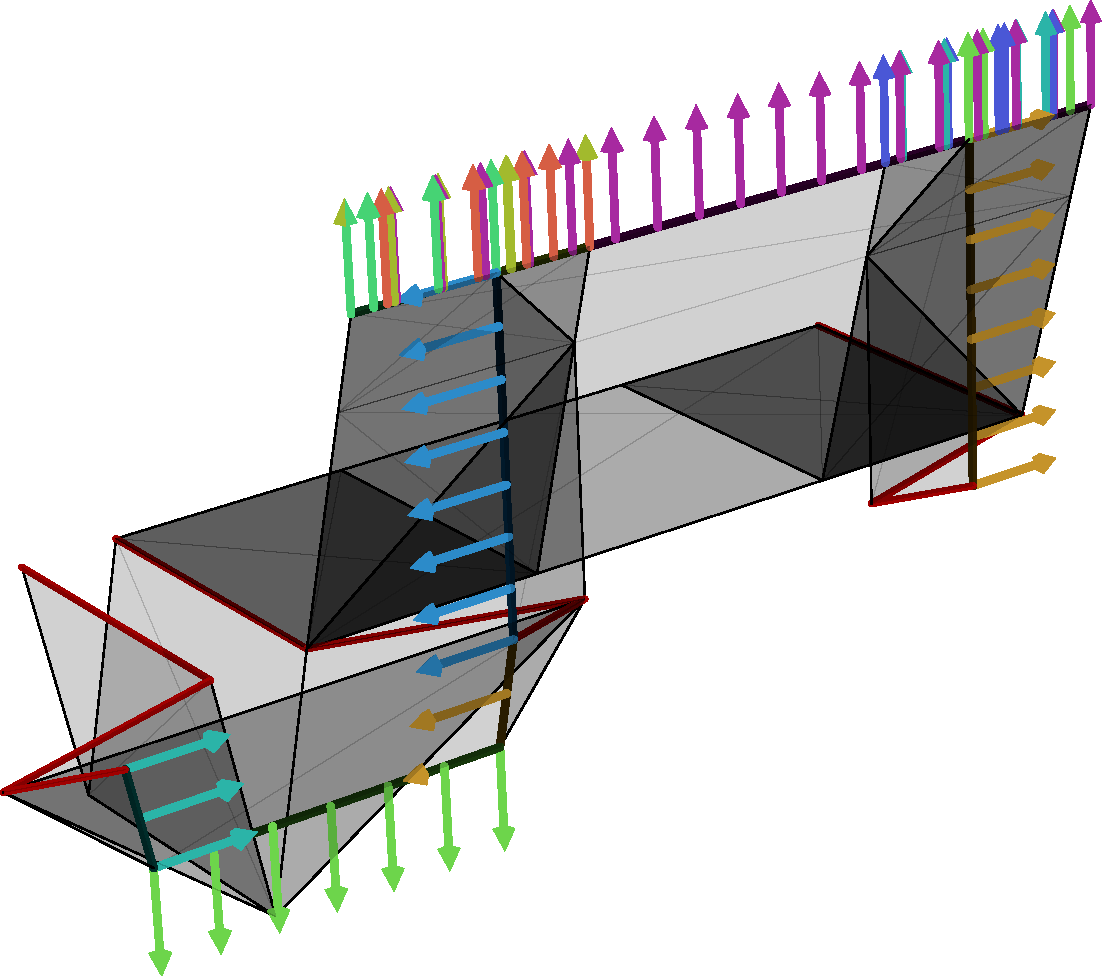
\includegraphics[width=0.23\textwidth]{figures/column_connector/column4.pdf}
    %}
    %\subfloat[]{
        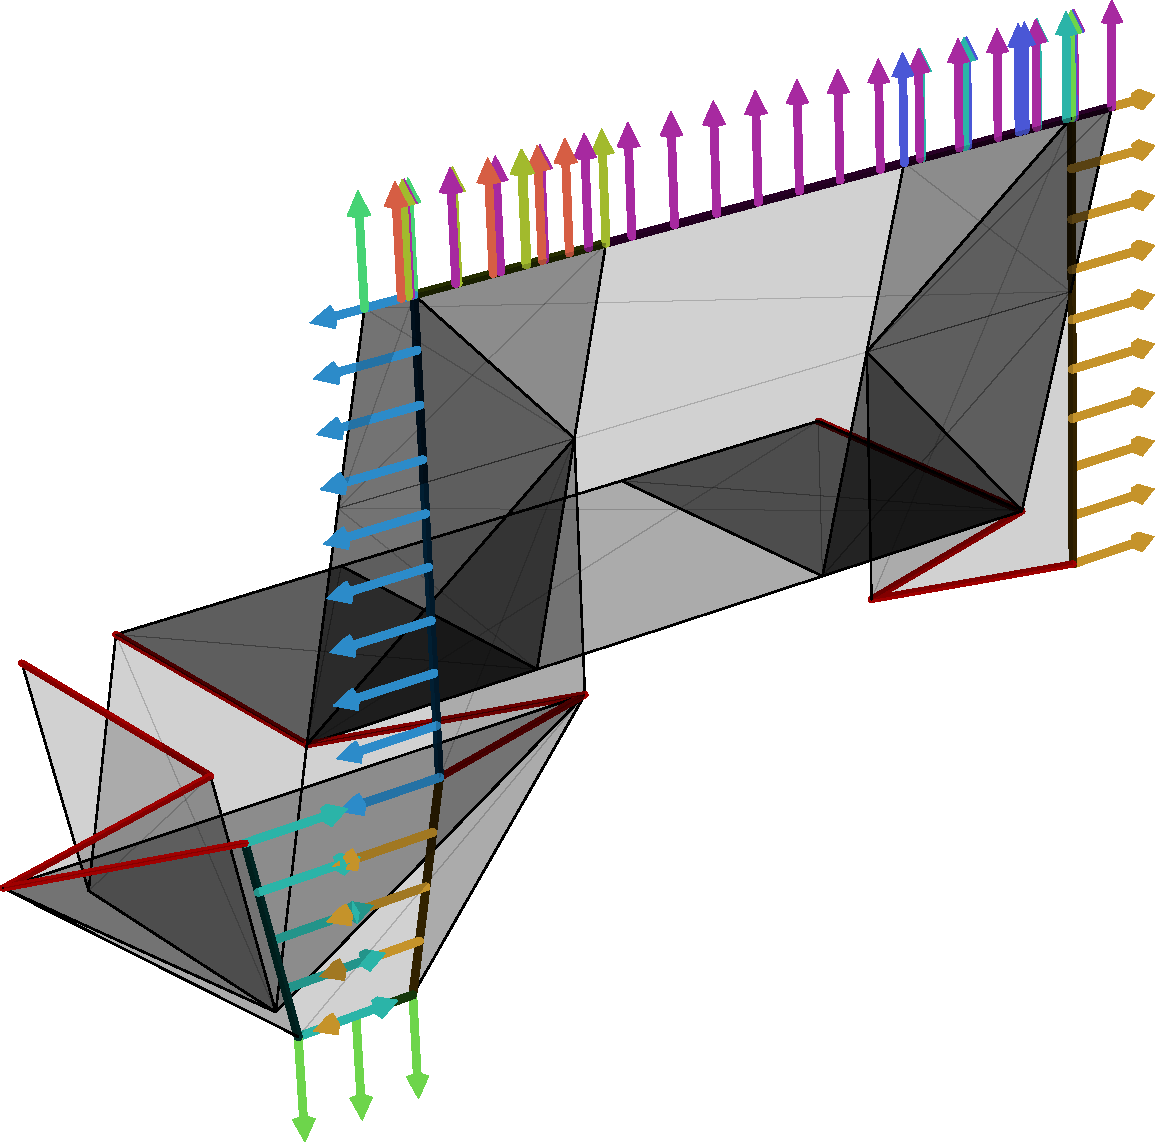
\includegraphics[width=0.23\textwidth]{figures/column_connector/column5.pdf}
    }%
    \subfloat[Back to \textbf{(a)}.]{
        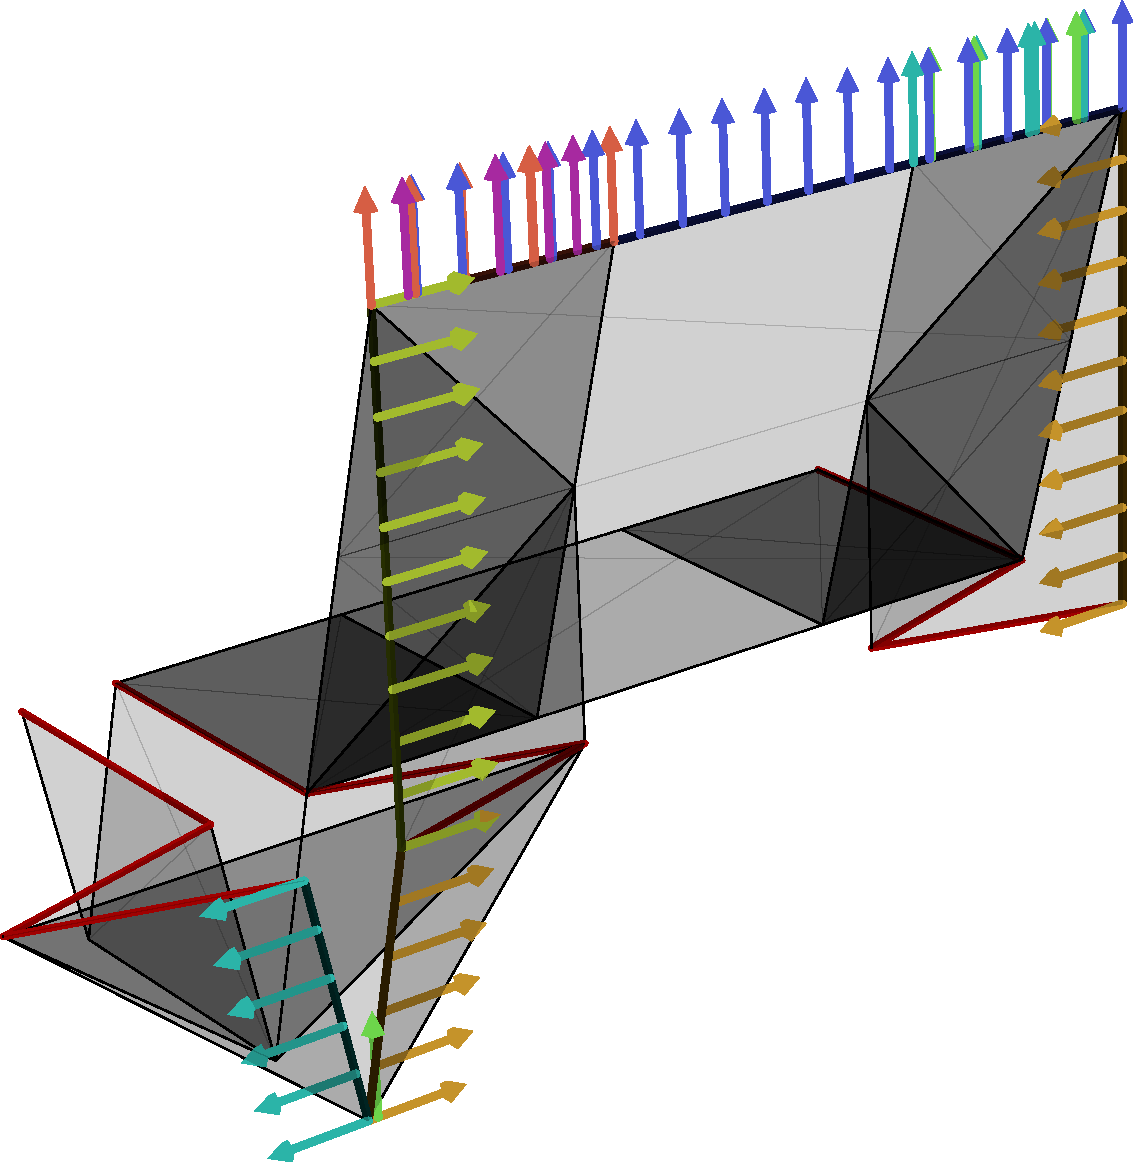
\includegraphics[width=0.23\textwidth]{figures/column_connector/column6.pdf}
    }%
    \subfloat[Same as \textbf{(b)}.]{
        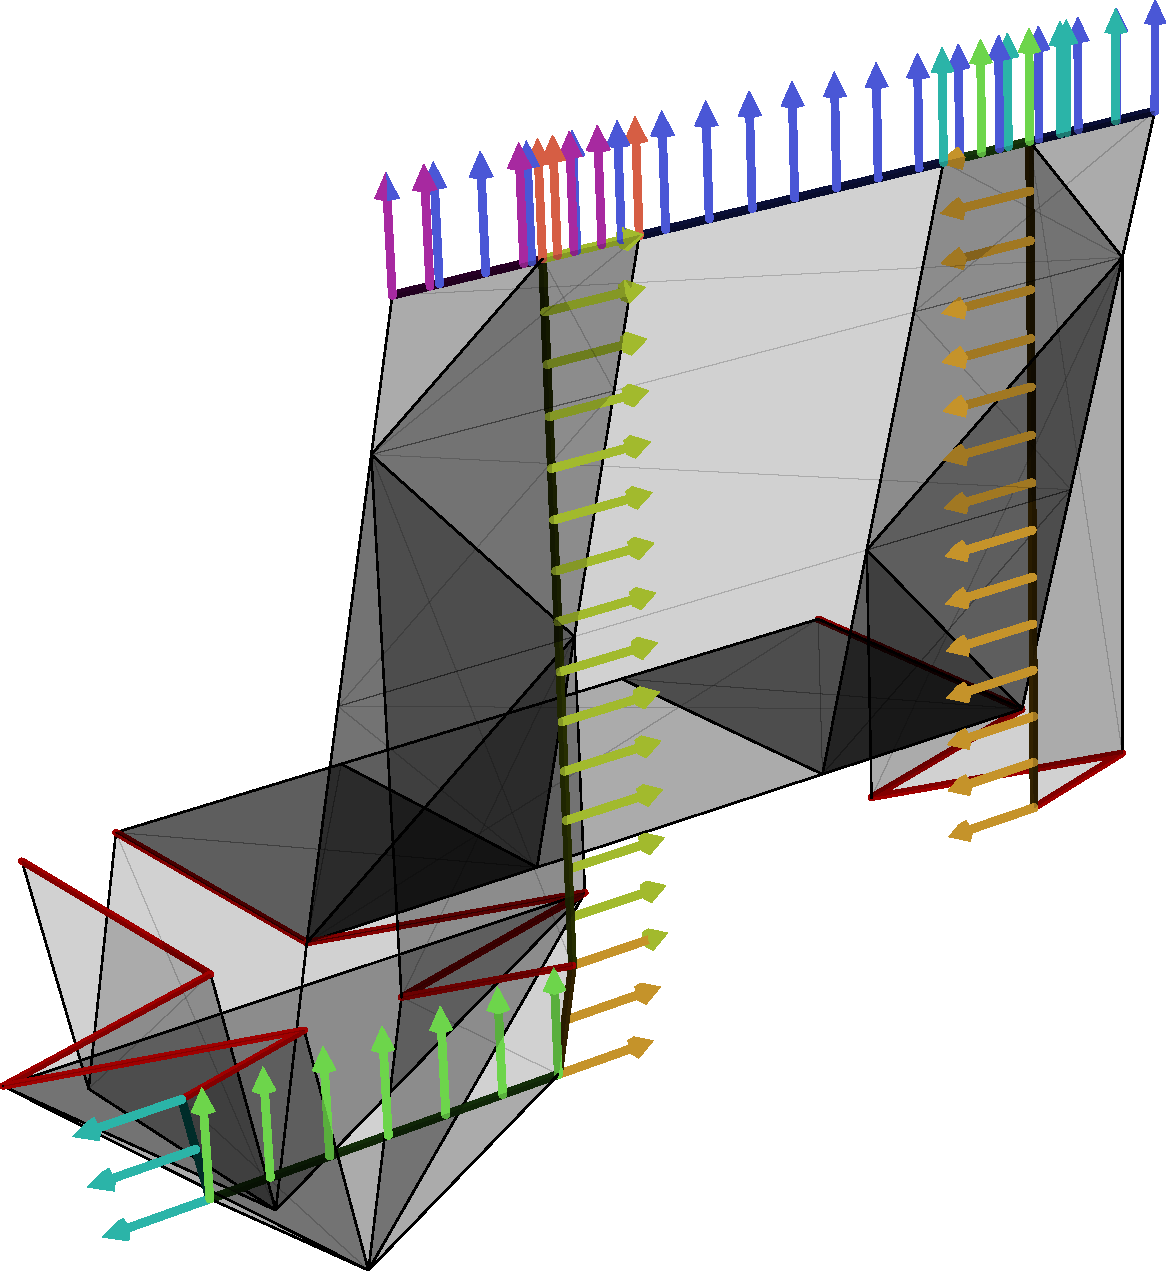
\includegraphics[width=0.23\textwidth]{figures/column_connector/column7.pdf}
    }%

    \subfloat[Same as \textbf{(d)}.]{
        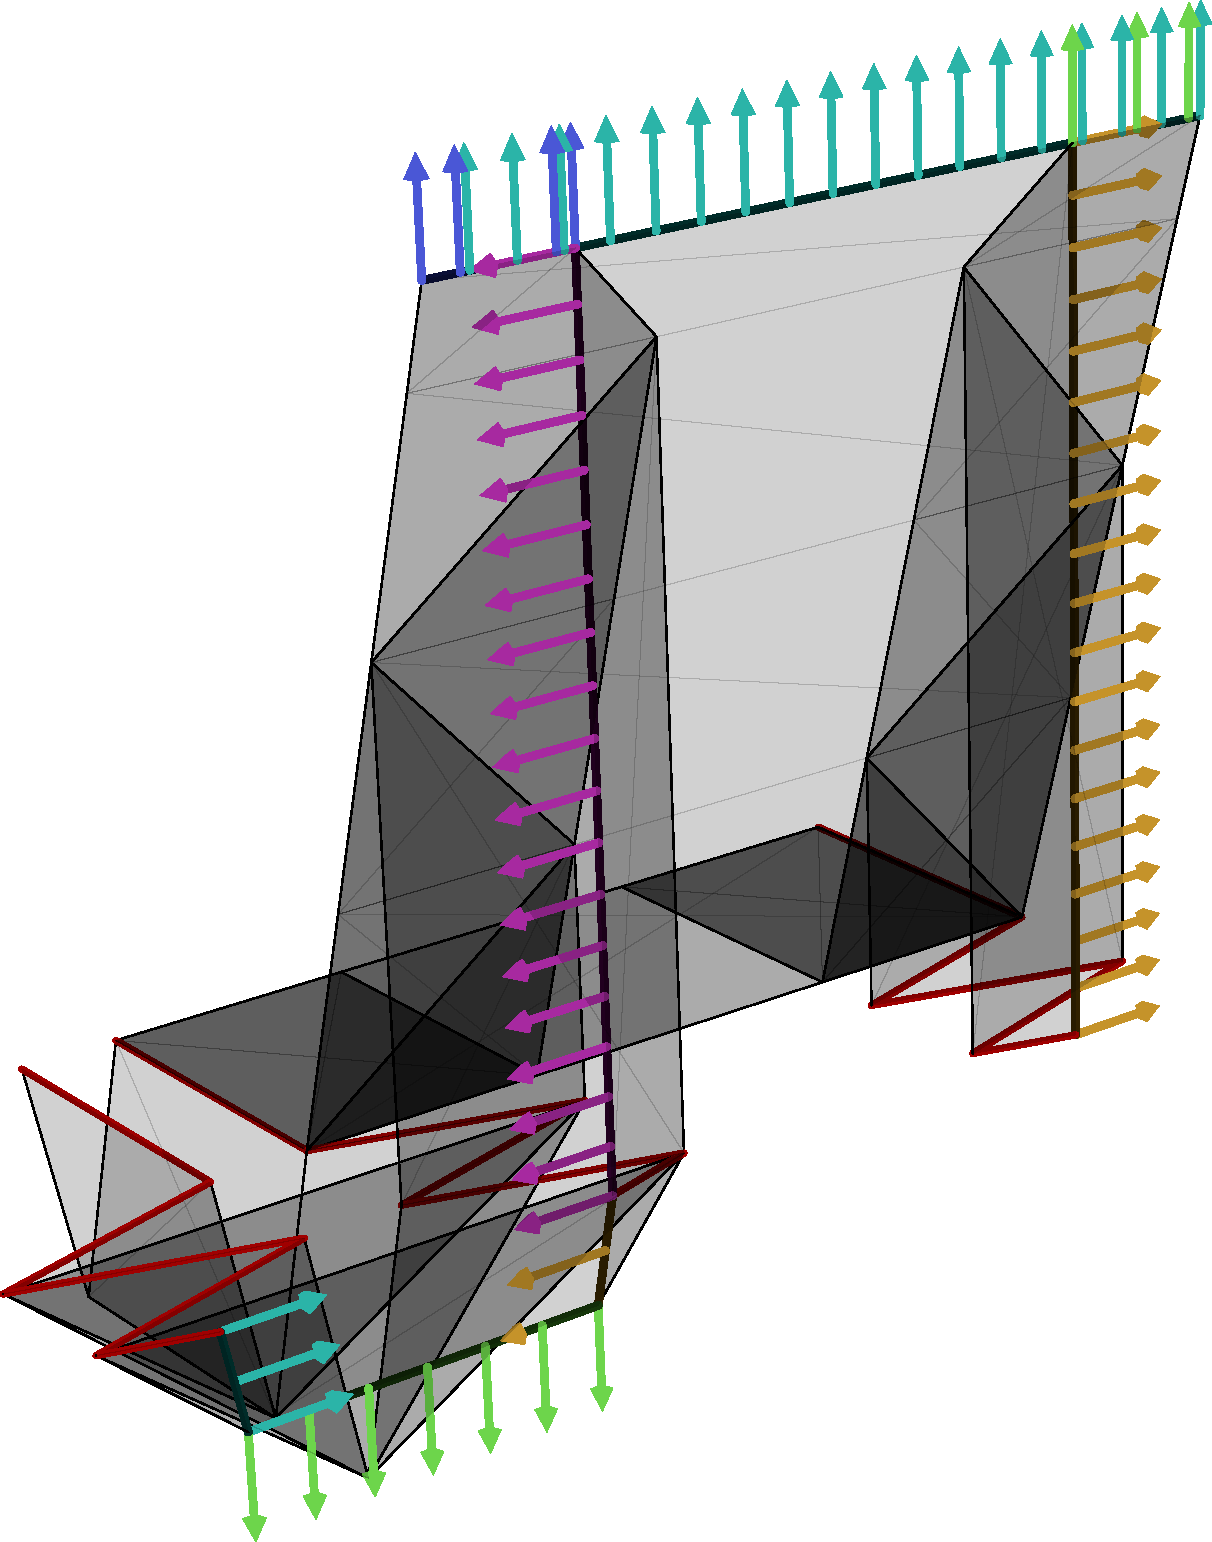
\includegraphics[width=0.29\textwidth]{figures/column_connector/column8.pdf}
    }%
    \subfloat[Level shift complete, and next level continues.]{
        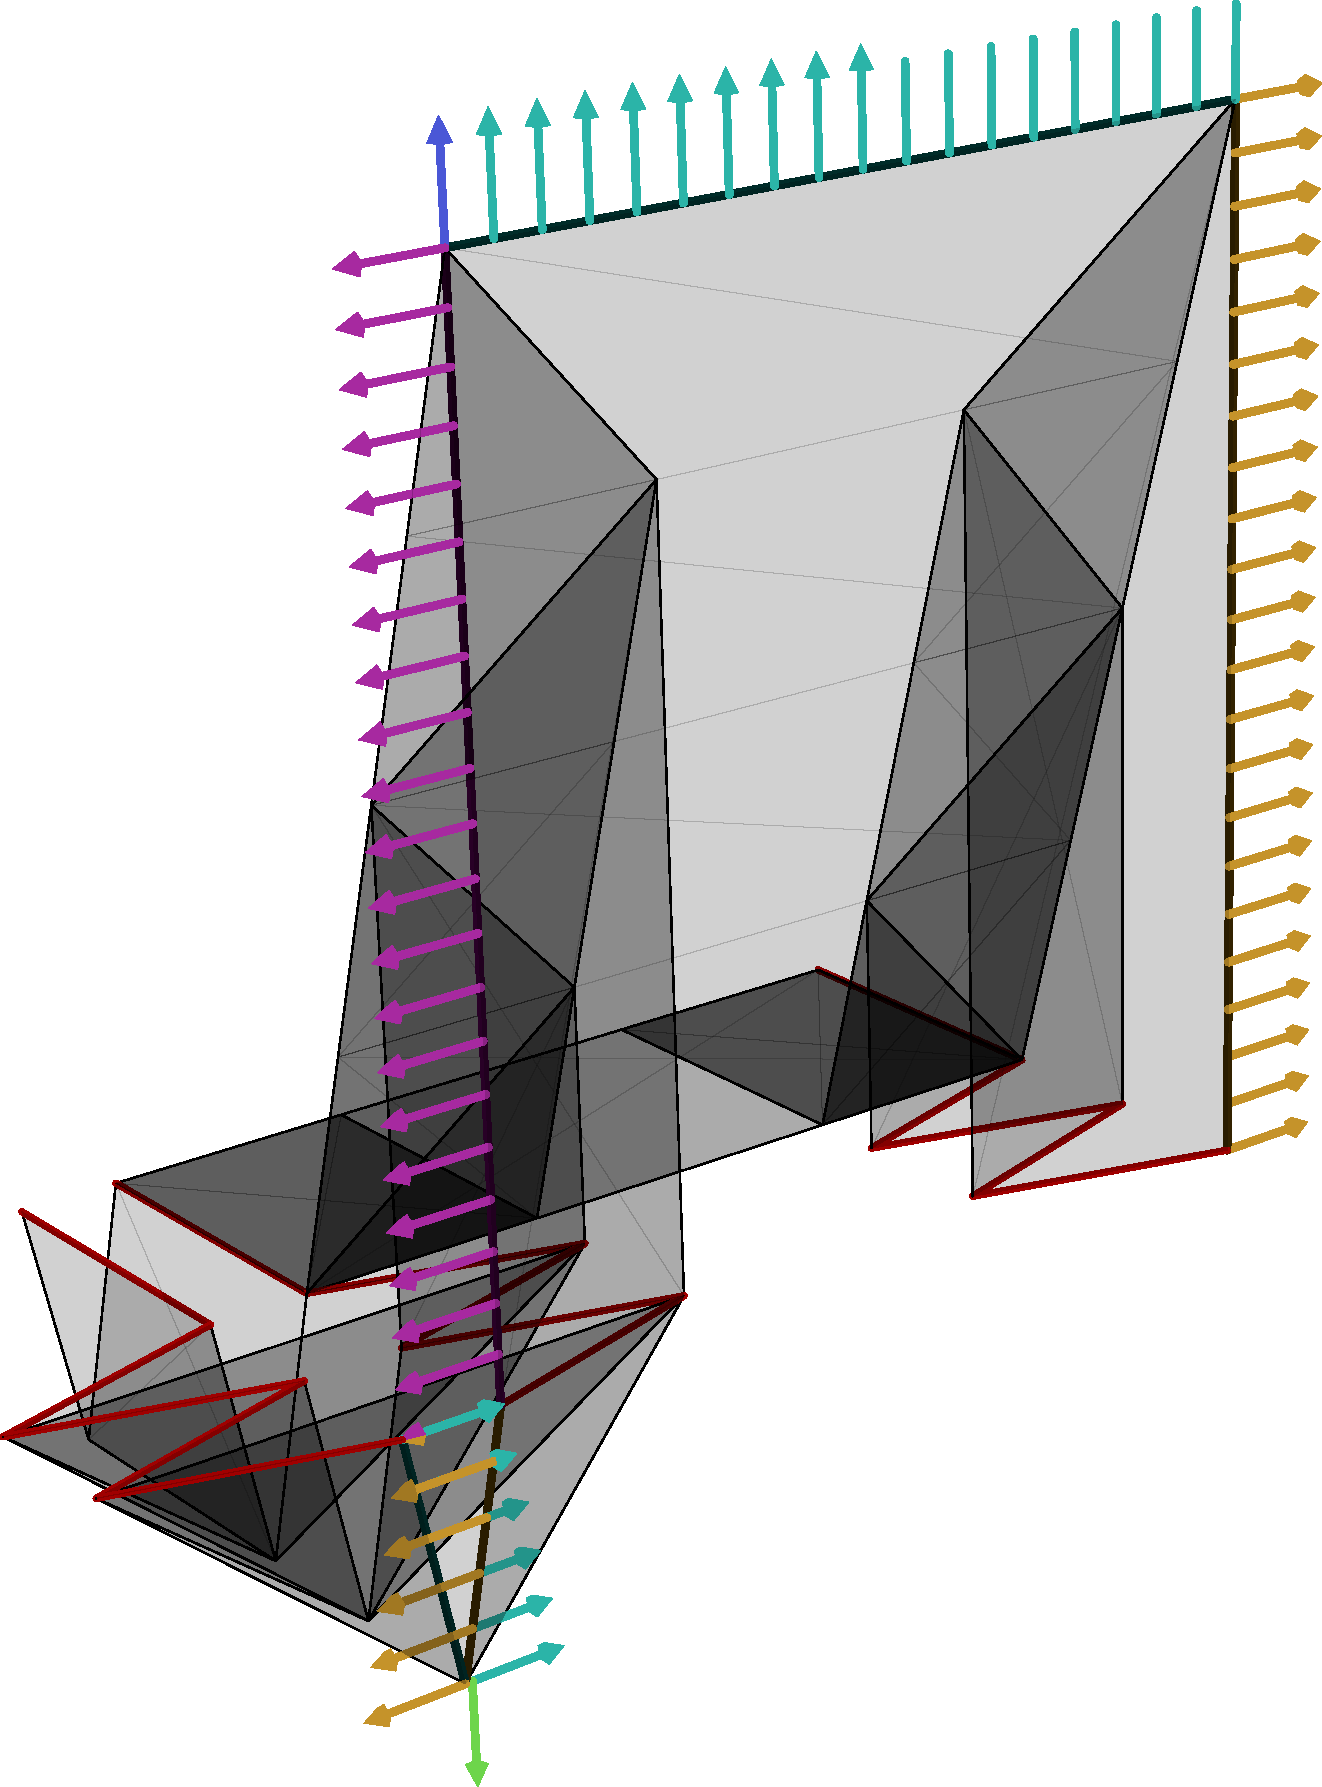
\includegraphics[width=0.29\textwidth]{figures/column_connector/column9.pdf}
    %}
    %\subfloat[Column and connector]{
        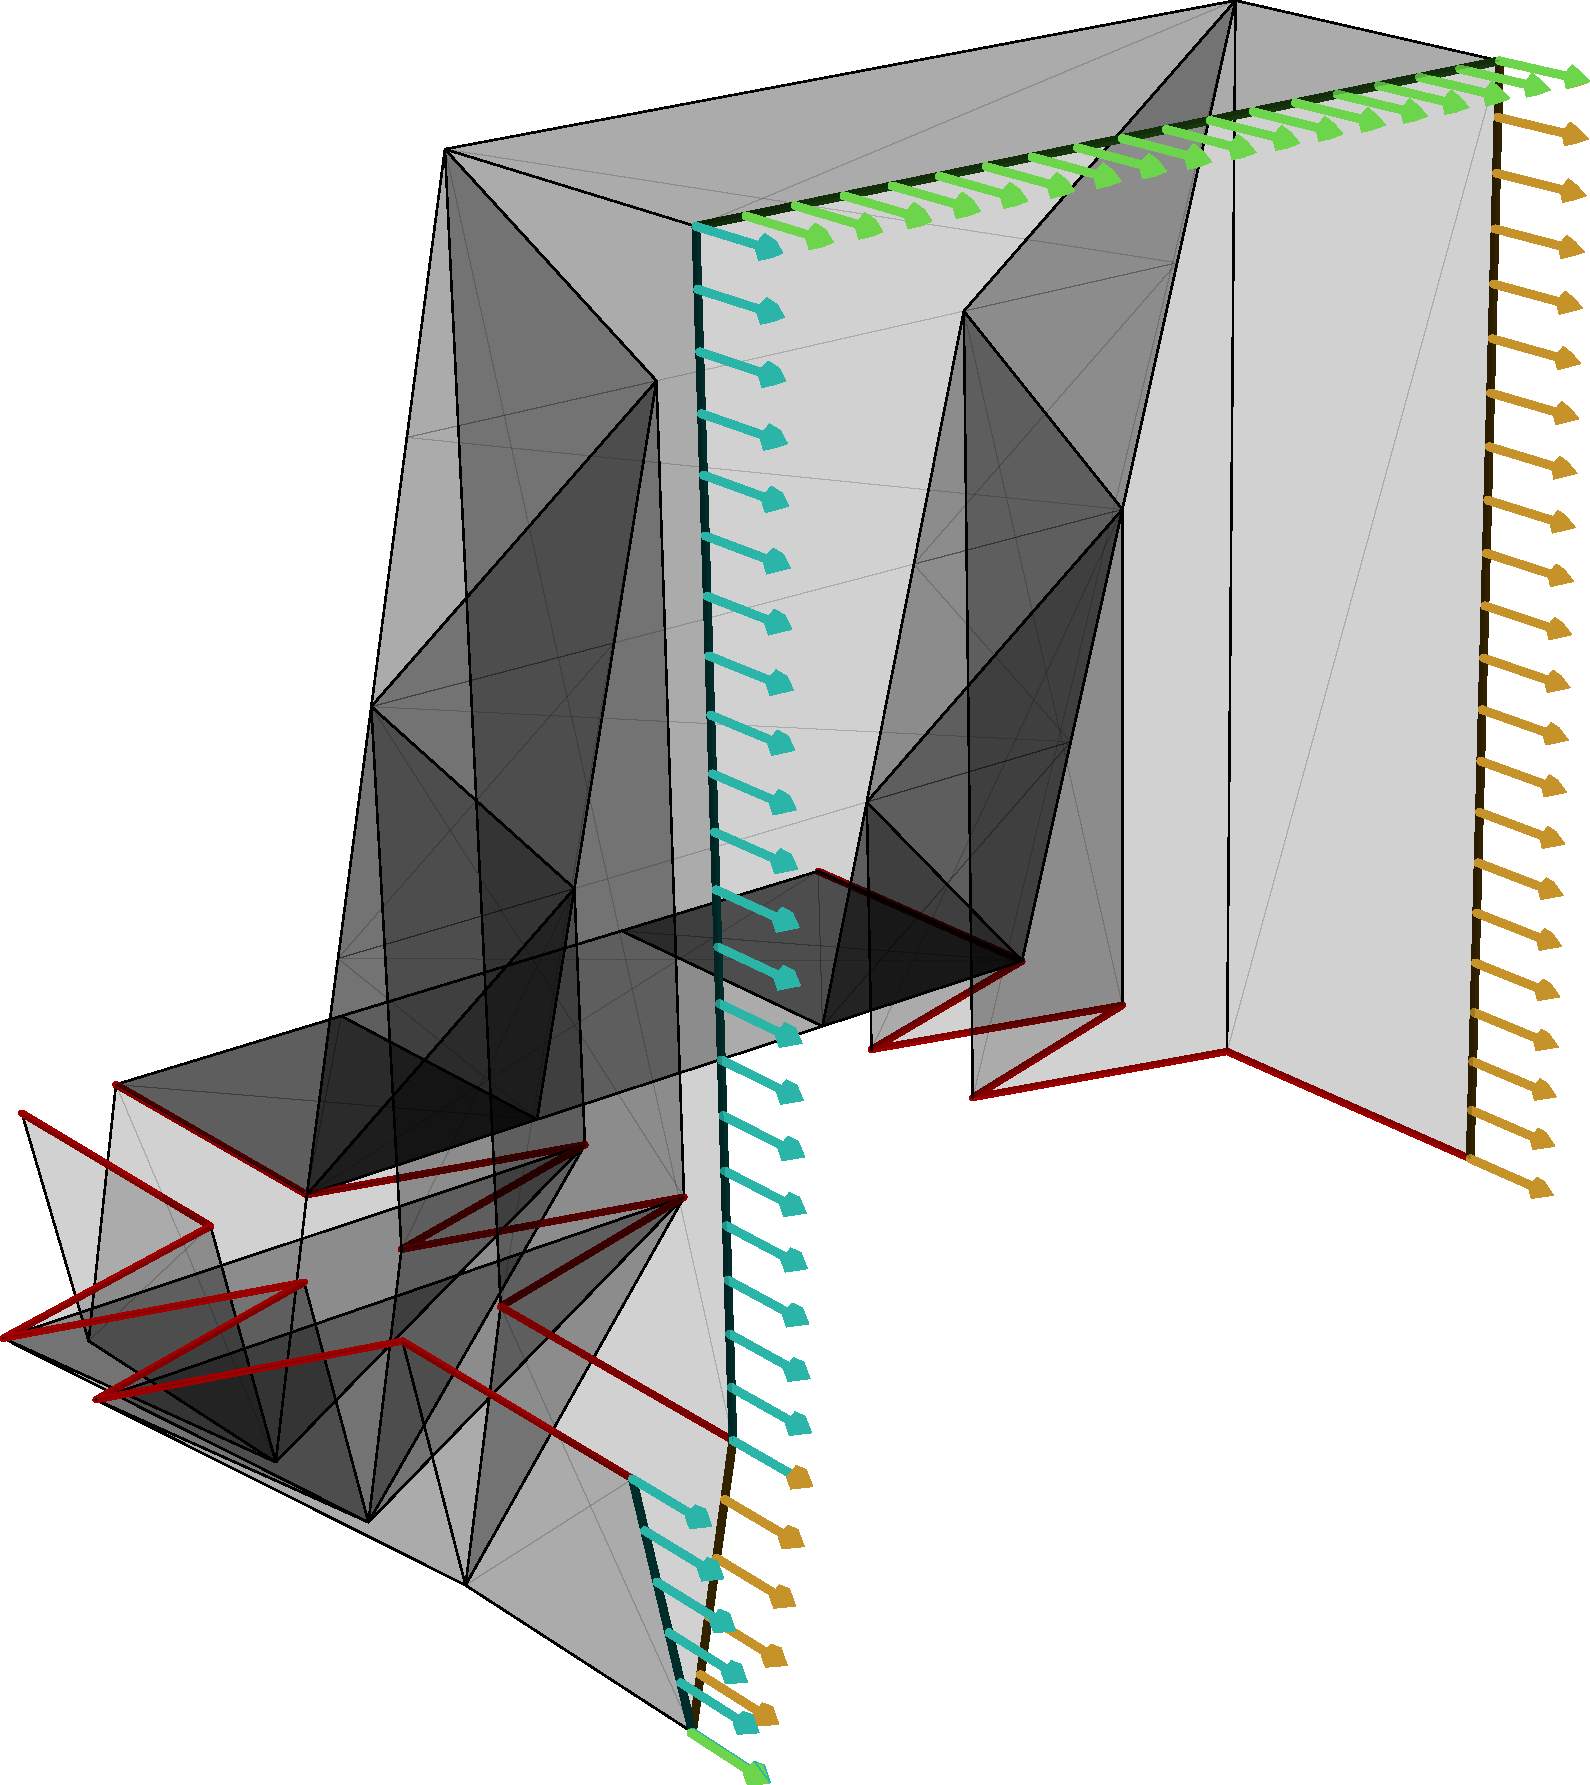
\includegraphics[width=0.34\textwidth]{figures/column_connector/column11.pdf}
    }%

    \subfloat[Connector gadget.]{
        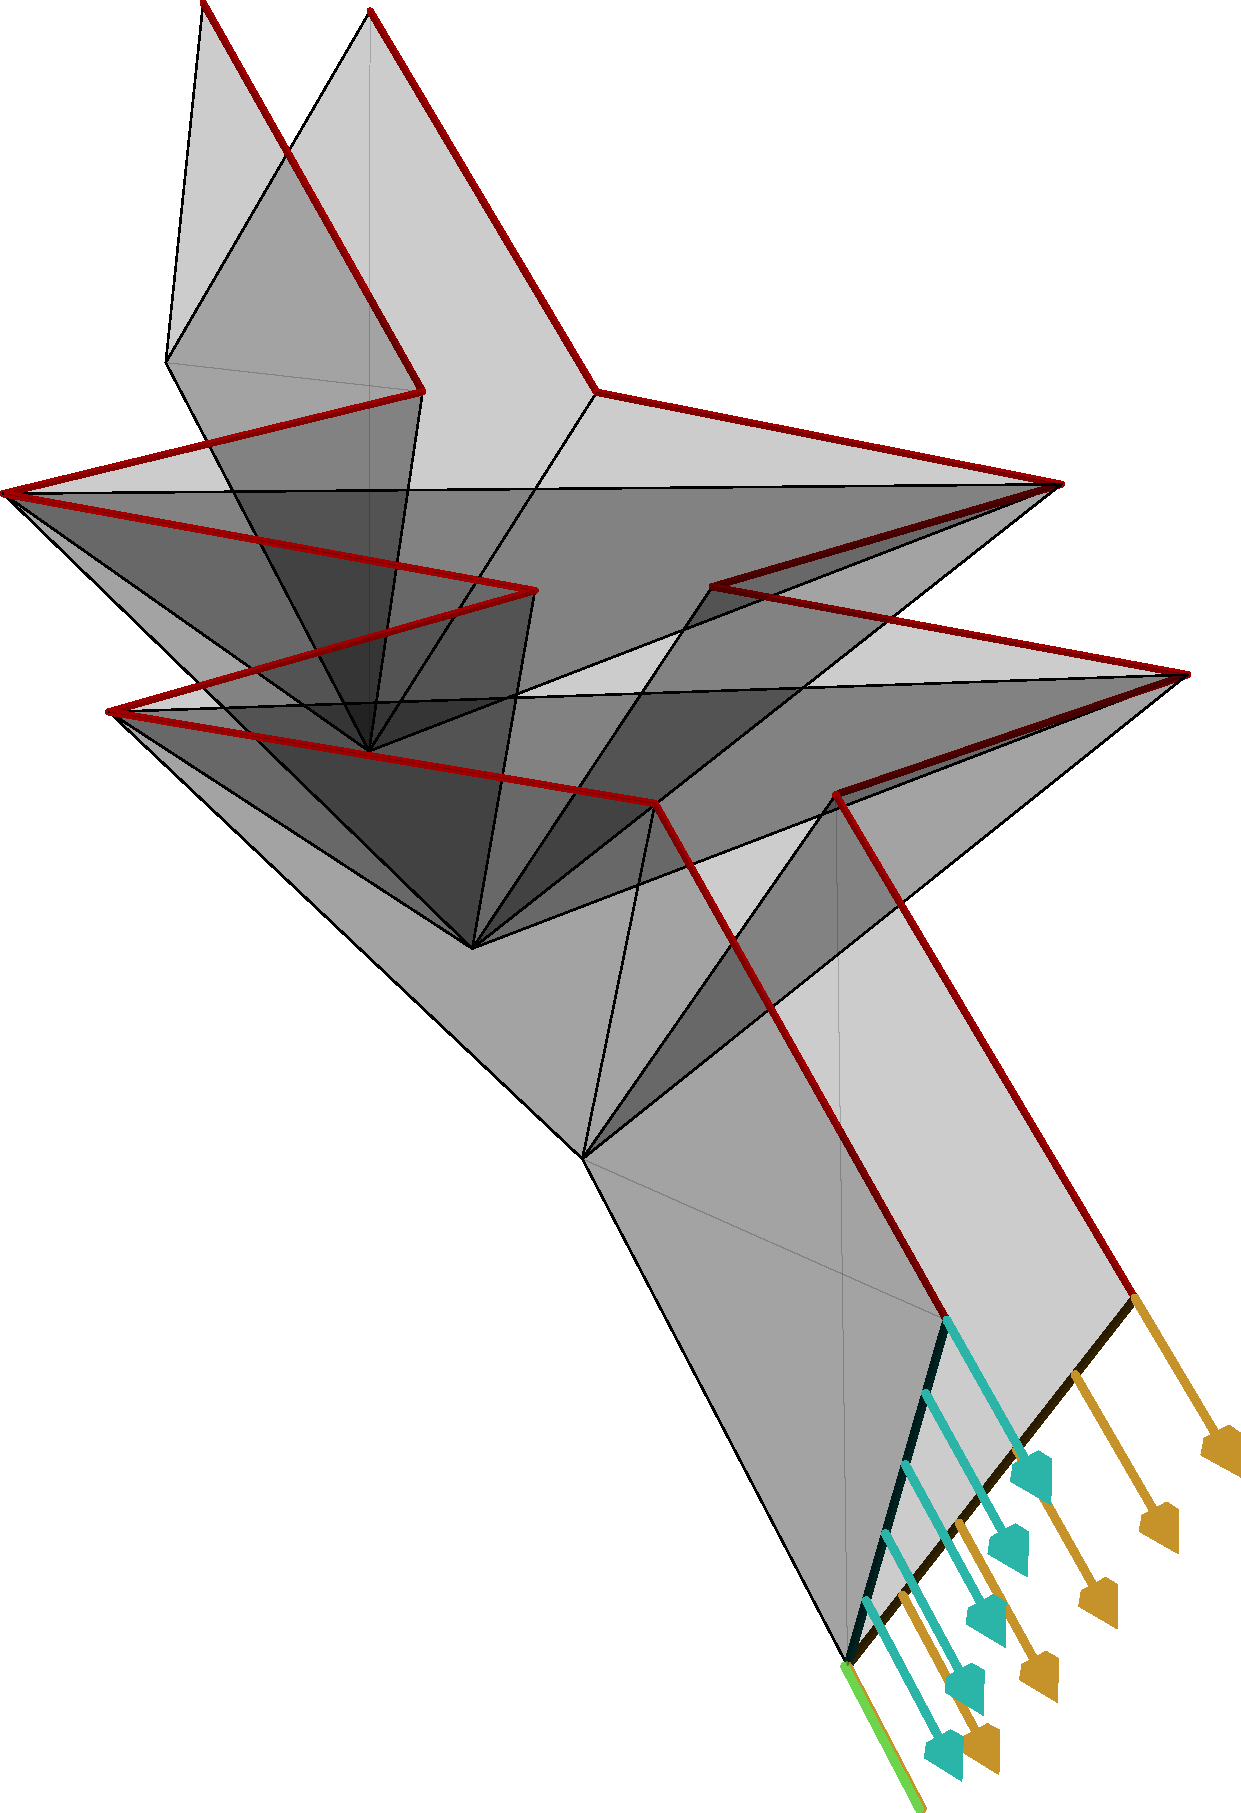
\includegraphics[width=0.31\textwidth]{figures/column_connector/connector0.pdf}
    }%
    \subfloat[Side view.]{
        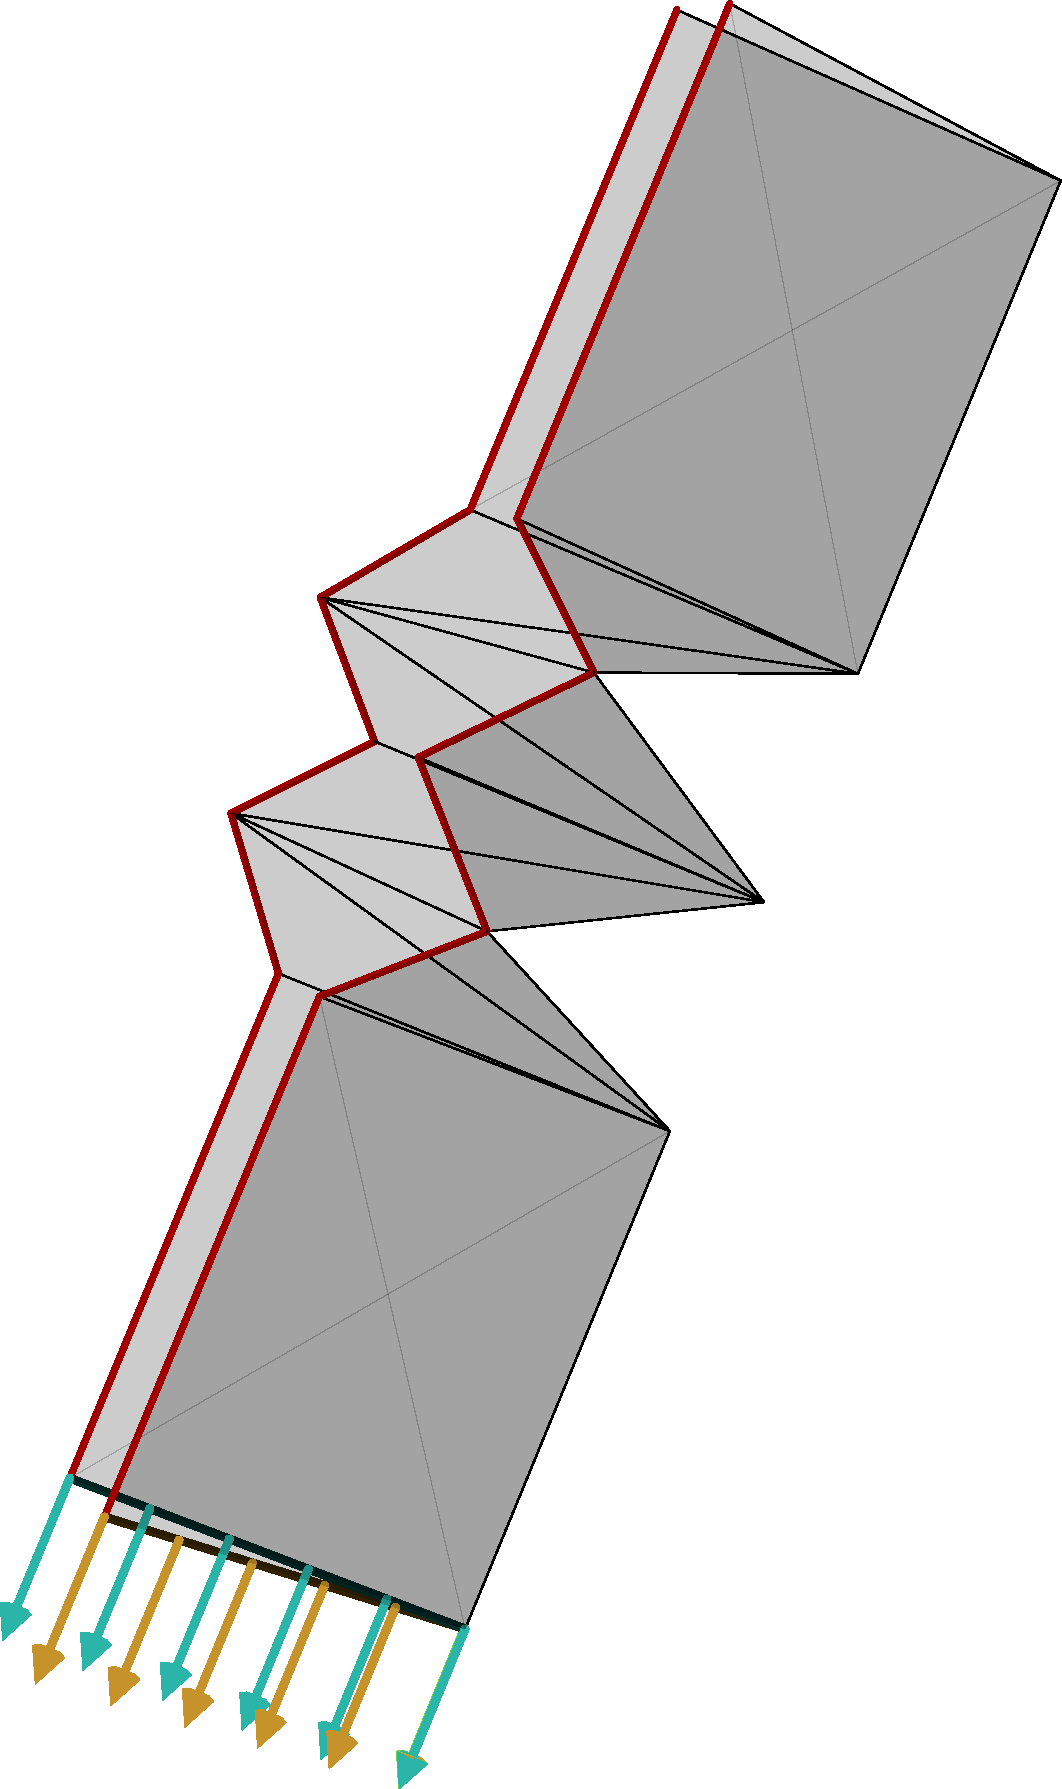
\includegraphics[width=0.27\textwidth]{figures/column_connector/connector1.pdf}
    }%
    \subfloat[Flat folded state.]{
        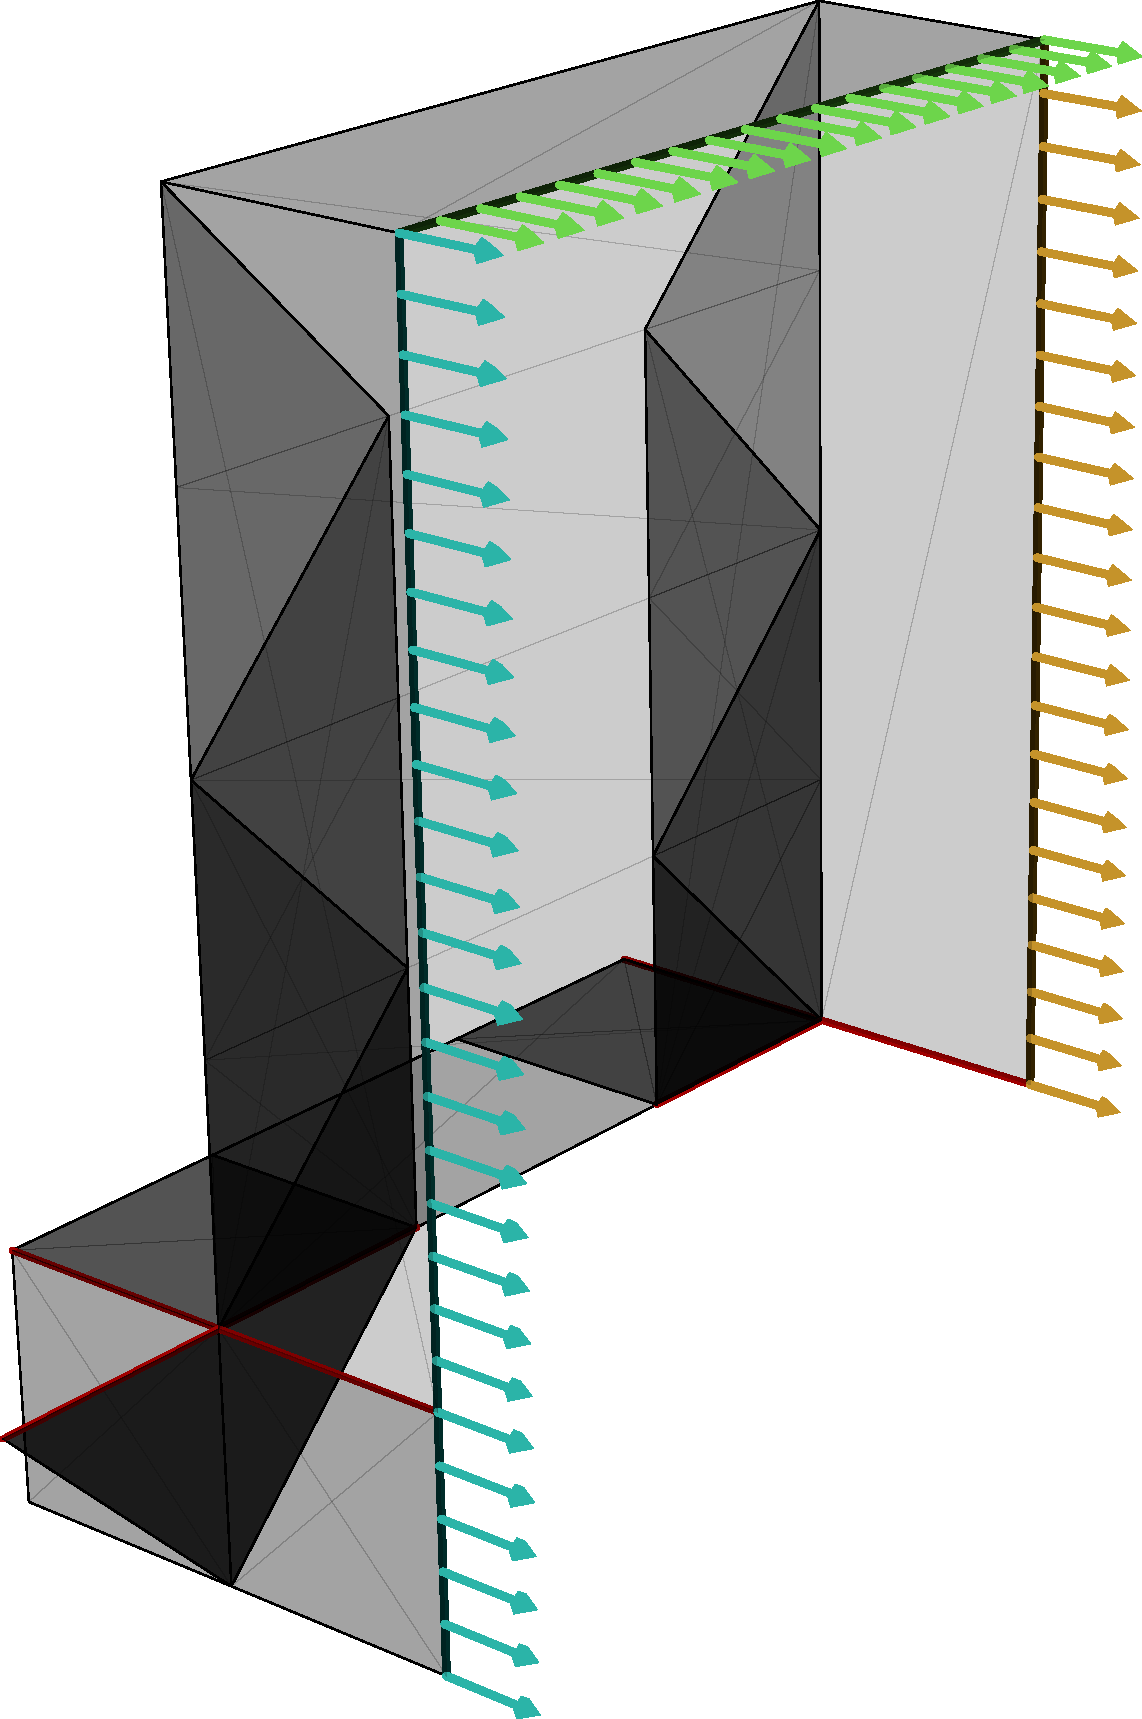
\includegraphics[width=0.31\textwidth]{figures/column_connector/column_connector0.pdf}
    }%
    \caption{
    Column gadget attached to a single column connector gadget.
    The red line demarcates the interface between the two gadgets.
    }
    \label{fig:column_connector}
    \vspace{-20pt}
\end{figure}
\clearpage


%\subsubsection{Alignment with Level Shifts}
%\label{sec:alignment_with_level_shifts}
